\documentclass[]{article}
\usepackage{lmodern}
\usepackage{amssymb,amsmath}
\usepackage{ifxetex,ifluatex}
\usepackage{fixltx2e} % provides \textsubscript
\ifnum 0\ifxetex 1\fi\ifluatex 1\fi=0 % if pdftex
  \usepackage[T1]{fontenc}
  \usepackage[utf8]{inputenc}
\else % if luatex or xelatex
  \ifxetex
    \usepackage{mathspec}
  \else
    \usepackage{fontspec}
  \fi
  \defaultfontfeatures{Ligatures=TeX,Scale=MatchLowercase}
\fi
% use upquote if available, for straight quotes in verbatim environments
\IfFileExists{upquote.sty}{\usepackage{upquote}}{}
% use microtype if available
\IfFileExists{microtype.sty}{%
\usepackage{microtype}
\UseMicrotypeSet[protrusion]{basicmath} % disable protrusion for tt fonts
}{}
\usepackage[margin=1in]{geometry}
\usepackage{hyperref}
\hypersetup{unicode=true,
            pdftitle={Regression Analysis},
            pdfauthor={Rhian Davies},
            pdfborder={0 0 0},
            breaklinks=true}
\urlstyle{same}  % don't use monospace font for urls
\usepackage{color}
\usepackage{fancyvrb}
\newcommand{\VerbBar}{|}
\newcommand{\VERB}{\Verb[commandchars=\\\{\}]}
\DefineVerbatimEnvironment{Highlighting}{Verbatim}{commandchars=\\\{\}}
% Add ',fontsize=\small' for more characters per line
\usepackage{framed}
\definecolor{shadecolor}{RGB}{248,248,248}
\newenvironment{Shaded}{\begin{snugshade}}{\end{snugshade}}
\newcommand{\KeywordTok}[1]{\textcolor[rgb]{0.13,0.29,0.53}{\textbf{{#1}}}}
\newcommand{\DataTypeTok}[1]{\textcolor[rgb]{0.13,0.29,0.53}{{#1}}}
\newcommand{\DecValTok}[1]{\textcolor[rgb]{0.00,0.00,0.81}{{#1}}}
\newcommand{\BaseNTok}[1]{\textcolor[rgb]{0.00,0.00,0.81}{{#1}}}
\newcommand{\FloatTok}[1]{\textcolor[rgb]{0.00,0.00,0.81}{{#1}}}
\newcommand{\ConstantTok}[1]{\textcolor[rgb]{0.00,0.00,0.00}{{#1}}}
\newcommand{\CharTok}[1]{\textcolor[rgb]{0.31,0.60,0.02}{{#1}}}
\newcommand{\SpecialCharTok}[1]{\textcolor[rgb]{0.00,0.00,0.00}{{#1}}}
\newcommand{\StringTok}[1]{\textcolor[rgb]{0.31,0.60,0.02}{{#1}}}
\newcommand{\VerbatimStringTok}[1]{\textcolor[rgb]{0.31,0.60,0.02}{{#1}}}
\newcommand{\SpecialStringTok}[1]{\textcolor[rgb]{0.31,0.60,0.02}{{#1}}}
\newcommand{\ImportTok}[1]{{#1}}
\newcommand{\CommentTok}[1]{\textcolor[rgb]{0.56,0.35,0.01}{\textit{{#1}}}}
\newcommand{\DocumentationTok}[1]{\textcolor[rgb]{0.56,0.35,0.01}{\textbf{\textit{{#1}}}}}
\newcommand{\AnnotationTok}[1]{\textcolor[rgb]{0.56,0.35,0.01}{\textbf{\textit{{#1}}}}}
\newcommand{\CommentVarTok}[1]{\textcolor[rgb]{0.56,0.35,0.01}{\textbf{\textit{{#1}}}}}
\newcommand{\OtherTok}[1]{\textcolor[rgb]{0.56,0.35,0.01}{{#1}}}
\newcommand{\FunctionTok}[1]{\textcolor[rgb]{0.00,0.00,0.00}{{#1}}}
\newcommand{\VariableTok}[1]{\textcolor[rgb]{0.00,0.00,0.00}{{#1}}}
\newcommand{\ControlFlowTok}[1]{\textcolor[rgb]{0.13,0.29,0.53}{\textbf{{#1}}}}
\newcommand{\OperatorTok}[1]{\textcolor[rgb]{0.81,0.36,0.00}{\textbf{{#1}}}}
\newcommand{\BuiltInTok}[1]{{#1}}
\newcommand{\ExtensionTok}[1]{{#1}}
\newcommand{\PreprocessorTok}[1]{\textcolor[rgb]{0.56,0.35,0.01}{\textit{{#1}}}}
\newcommand{\AttributeTok}[1]{\textcolor[rgb]{0.77,0.63,0.00}{{#1}}}
\newcommand{\RegionMarkerTok}[1]{{#1}}
\newcommand{\InformationTok}[1]{\textcolor[rgb]{0.56,0.35,0.01}{\textbf{\textit{{#1}}}}}
\newcommand{\WarningTok}[1]{\textcolor[rgb]{0.56,0.35,0.01}{\textbf{\textit{{#1}}}}}
\newcommand{\AlertTok}[1]{\textcolor[rgb]{0.94,0.16,0.16}{{#1}}}
\newcommand{\ErrorTok}[1]{\textcolor[rgb]{0.64,0.00,0.00}{\textbf{{#1}}}}
\newcommand{\NormalTok}[1]{{#1}}
\usepackage{graphicx,grffile}
\makeatletter
\def\maxwidth{\ifdim\Gin@nat@width>\linewidth\linewidth\else\Gin@nat@width\fi}
\def\maxheight{\ifdim\Gin@nat@height>\textheight\textheight\else\Gin@nat@height\fi}
\makeatother
% Scale images if necessary, so that they will not overflow the page
% margins by default, and it is still possible to overwrite the defaults
% using explicit options in \includegraphics[width, height, ...]{}
\setkeys{Gin}{width=\maxwidth,height=\maxheight,keepaspectratio}
\IfFileExists{parskip.sty}{%
\usepackage{parskip}
}{% else
\setlength{\parindent}{0pt}
\setlength{\parskip}{6pt plus 2pt minus 1pt}
}
\setlength{\emergencystretch}{3em}  % prevent overfull lines
\providecommand{\tightlist}{%
  \setlength{\itemsep}{0pt}\setlength{\parskip}{0pt}}
\setcounter{secnumdepth}{0}
% Redefines (sub)paragraphs to behave more like sections
\ifx\paragraph\undefined\else
\let\oldparagraph\paragraph
\renewcommand{\paragraph}[1]{\oldparagraph{#1}\mbox{}}
\fi
\ifx\subparagraph\undefined\else
\let\oldsubparagraph\subparagraph
\renewcommand{\subparagraph}[1]{\oldsubparagraph{#1}\mbox{}}
\fi

%%% Use protect on footnotes to avoid problems with footnotes in titles
\let\rmarkdownfootnote\footnote%
\def\footnote{\protect\rmarkdownfootnote}

%%% Change title format to be more compact
\usepackage{titling}

% Create subtitle command for use in maketitle
\newcommand{\subtitle}[1]{
  \posttitle{
    \begin{center}\large#1\end{center}
    }
}

\setlength{\droptitle}{-2em}
  \title{Regression Analysis}
  \pretitle{\vspace{\droptitle}\centering\huge}
  \posttitle{\par}
  \author{Rhian Davies}
  \preauthor{\centering\large\emph}
  \postauthor{\par}
  \date{}
  \predate{}\postdate{}


\begin{document}
\maketitle

\subsection{Preproccesing}\label{preproccesing}

\begin{itemize}
\tightlist
\item
  Read in raw data.
\item
  Consider only 12 month policies.
\item
  Exclude any expensive cars (\textgreater{} £30,000)
\item
  Exclude any cars with engine size \textgreater{} 4L
\end{itemize}

We exclude any very expensive cars and high engine cars from the data
set. This is because they might be outliers (some very suspicious
values). Also removing these points allows us to visualise the rest of
the data more easily. By excluding all cars \textgreater{} £30,000 or
with an engine size \textgreater{} 4000, we remove 1056 quotes
(\textasciitilde{}0.5\% of the 12 month quotes.)

\subsection{Transformations}\label{transformations}

We apply a log transform to the Expected Value. Clustream streaming
seems to been having issues with Expected Value of Car unless I
transform it with log or sqrt or similar.

\includegraphics{offline_regression_files/figure-latex/fig.hold-1.pdf}
\includegraphics{offline_regression_files/figure-latex/fig.hold-2.pdf}

\subsection{Regression on the full
dataset}\label{regression-on-the-full-dataset}

The R function step() can be used to perform variable selection. To
perform forward selection we need to begin by specifying a starting
model and the range of models which we want to examine in the search.

We can perform forward selection. This tells R to start with the null
model and search through models lying in the range between the null and
full model using the forward selection algorithm. It gives rise to the
following output:

\begin{Shaded}
\begin{Highlighting}[]
\NormalTok{null=}\KeywordTok{lm}\NormalTok{(Value_B~}\DecValTok{1}\NormalTok{, }\DataTypeTok{data=}\NormalTok{Data)}
\NormalTok{full=}\KeywordTok{lm}\NormalTok{(Value_B~., }\DataTypeTok{data=}\NormalTok{Data)}
\KeywordTok{step}\NormalTok{(null, }\DataTypeTok{scope=}\KeywordTok{list}\NormalTok{(}\DataTypeTok{lower=}\NormalTok{null, }\DataTypeTok{upper=}\NormalTok{full), }\DataTypeTok{direction=}\StringTok{"forward"}\NormalTok{)}
\end{Highlighting}
\end{Shaded}

\begin{verbatim}
## Start:  AIC=1823561
## Value_B ~ 1
## 
##                         Df Sum of Sq       RSS     AIC
## + CC                     1  41139084 444443753 1802363
## + Age_of_Car             1  15105732 470477105 1815995
## + Age_of_Driver          1   9774717 475808119 1818694
## + Expected_Value_of_Car  1   2329961 483252876 1822412
## <none>                               485582837 1823561
## 
## Step:  AIC=1802363
## Value_B ~ CC
## 
##                         Df Sum of Sq       RSS     AIC
## + Age_of_Car             1  16913380 427530373 1793074
## + Expected_Value_of_Car  1  15131262 429312491 1794070
## + Age_of_Driver          1   6030858 438412896 1799093
## <none>                               444443753 1802363
## 
## Step:  AIC=1793074
## Value_B ~ CC + Age_of_Car
## 
##                         Df Sum of Sq       RSS     AIC
## + Age_of_Driver          1   2873539 424656835 1791461
## + Expected_Value_of_Car  1    431065 427099308 1792834
## <none>                               427530373 1793074
## 
## Step:  AIC=1791461
## Value_B ~ CC + Age_of_Car + Age_of_Driver
## 
##                         Df Sum of Sq       RSS     AIC
## + Expected_Value_of_Car  1    484489 424172346 1791189
## <none>                               424656835 1791461
## 
## Step:  AIC=1791189
## Value_B ~ CC + Age_of_Car + Age_of_Driver + Expected_Value_of_Car
\end{verbatim}

\begin{verbatim}
## 
## Call:
## lm(formula = Value_B ~ CC + Age_of_Car + Age_of_Driver + Expected_Value_of_Car, 
##     data = Data)
## 
## Coefficients:
##           (Intercept)                     CC             Age_of_Car  
##             191.39042                0.04399                1.00745  
##         Age_of_Driver  Expected_Value_of_Car  
##               0.27747               -3.58568
\end{verbatim}

This indicates that we should use all possible predictors in our linear
model.

\begin{Shaded}
\begin{Highlighting}[]
\KeywordTok{anova}\NormalTok{(full)}
\end{Highlighting}
\end{Shaded}

\begin{verbatim}
## Analysis of Variance Table
## 
## Response: Value_B
##                           Df    Sum Sq  Mean Sq F value    Pr(>F)    
## Age_of_Driver              1   9774717  9774717  5518.5 < 2.2e-16 ***
## Age_of_Car                 1  11285490 11285490  6371.5 < 2.2e-16 ***
## Expected_Value_of_Car      1   7946822  7946822  4486.6 < 2.2e-16 ***
## CC                         1  32403462 32403462 18294.1 < 2.2e-16 ***
## Residuals             239476 424172346     1771                      
## ---
## Signif. codes:  0 '***' 0.001 '**' 0.01 '*' 0.05 '.' 0.1 ' ' 1
\end{verbatim}

\begin{Shaded}
\begin{Highlighting}[]
\KeywordTok{par}\NormalTok{(}\DataTypeTok{mfrow =} \KeywordTok{c}\NormalTok{(}\DecValTok{2}\NormalTok{,}\DecValTok{2}\NormalTok{))}
\KeywordTok{plot}\NormalTok{(full)}
\end{Highlighting}
\end{Shaded}

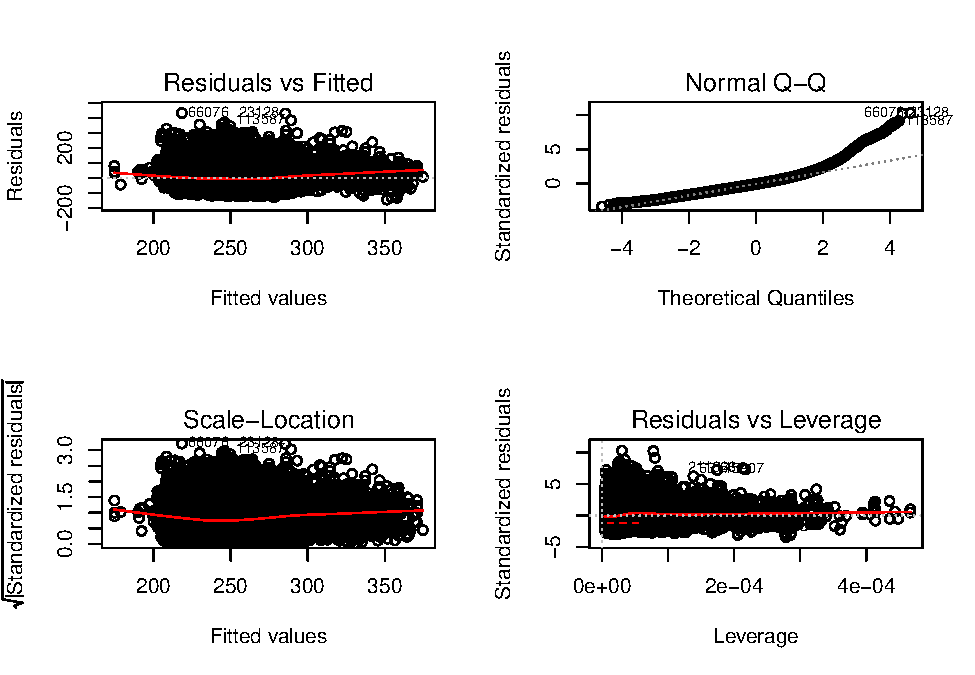
\includegraphics{offline_regression_files/figure-latex/unnamed-chunk-4-1.pdf}

We can also view the actual against predicted.

\begin{Shaded}
\begin{Highlighting}[]
\NormalTok{predicted =}\StringTok{ }\KeywordTok{predict}\NormalTok{(full, }\DataTypeTok{newdata =} \NormalTok{Data[,-}\DecValTok{5}\NormalTok{])}
\NormalTok{actual =}\StringTok{ }\NormalTok{Data[,}\DecValTok{5}\NormalTok{]}
\KeywordTok{plot}\NormalTok{(actual, predicted)}
\end{Highlighting}
\end{Shaded}

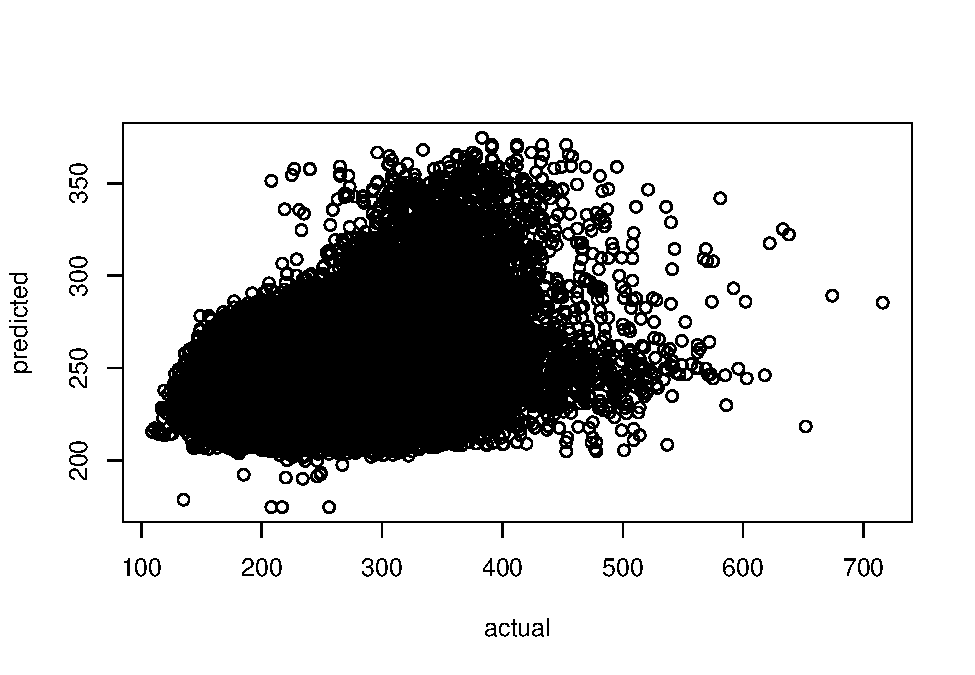
\includegraphics{offline_regression_files/figure-latex/unnamed-chunk-5-1.pdf}

This model isn't perfect but we will progress with it for now.

\subsubsection{Online Regression}\label{online-regression}

\begin{itemize}
\item
  Treat the dataset as a datastream
\item
  Initialise the clustream algorithm with 1000 data points.
\item
  Increment the data stream by 2000 points, tracking with Clustream
\item
  Use the clustream microcluster centers as input to a linear model
  (same set up as offline)
\item
  Store the coefficients from the model
\item
  Repeat the last 3 steps until the end of the stream
\end{itemize}

This procedure is carried it with the following three algorithms;
Clustream, weighted Clustream and a windowed approach.

We vary the nMicro clusters / window size used.

Using this we can plot how the coeffients change each time a linear
model is created.

\begin{Shaded}
\begin{Highlighting}[]
\NormalTok{results =}\StringTok{ }\KeywordTok{readRDS}\NormalTok{(}\DataTypeTok{file =} \StringTok{"../results/online_regression_results.RDS"}\NormalTok{)}

\NormalTok{results %>%}
\StringTok{  }\KeywordTok{filter}\NormalTok{(alg !=}\StringTok{ "offline"}\NormalTok{) %>%}
\StringTok{  }\KeywordTok{filter}\NormalTok{(nMicro ==}\StringTok{ }\DecValTok{500}\NormalTok{) %>%}
\StringTok{  }\CommentTok{#filter(alg == "online" | alg== "window" ) %>%}
\StringTok{  }\KeywordTok{ggplot}\NormalTok{(}\KeywordTok{aes}\NormalTok{(rep, Age_of_Car, }\DataTypeTok{col =} \NormalTok{alg)) +}
\StringTok{  }\KeywordTok{geom_line}\NormalTok{(}\DataTypeTok{size =} \FloatTok{1.2}\NormalTok{) +}
\StringTok{  }\KeywordTok{geom_hline}\NormalTok{(}\DataTypeTok{yintercept =} \KeywordTok{filter}\NormalTok{(results, alg ==}\StringTok{ "offline"}\NormalTok{)$Age_of_Car, }\DataTypeTok{size =} \DecValTok{1}\NormalTok{) +}\StringTok{ }
\StringTok{  }\KeywordTok{xlab}\NormalTok{(}\StringTok{"Time"}\NormalTok{)+}
\StringTok{  }\KeywordTok{ylab}\NormalTok{(}\StringTok{"Value"}\NormalTok{) +}
\StringTok{  }\KeywordTok{ggtitle}\NormalTok{(}\StringTok{"Age of Car Coeffient"}\NormalTok{) }
\end{Highlighting}
\end{Shaded}

\includegraphics{offline_regression_files/figure-latex/unnamed-chunk-6-1.pdf}

We can view how the coeffcients for all of the model predictors change
over time for different algorithms as shown in the plot above. However
this is messy to look at, and viewing the results for varying number of
microclusters would make things even more confusing.

Instead we focus on the absolute mean error from the coefficient given
in the offline model, and the variance of the coefficients.

\subsubsection{Mean Abs Error Plots}\label{mean-abs-error-plots}

\includegraphics{offline_regression_files/figure-latex/unnamed-chunk-7-1.pdf}
\includegraphics{offline_regression_files/figure-latex/unnamed-chunk-7-2.pdf}
\includegraphics{offline_regression_files/figure-latex/unnamed-chunk-7-3.pdf}
\includegraphics{offline_regression_files/figure-latex/unnamed-chunk-7-4.pdf}
\includegraphics{offline_regression_files/figure-latex/unnamed-chunk-7-5.pdf}

\subsubsection{Variance Plots}\label{variance-plots}

\includegraphics{offline_regression_files/figure-latex/unnamed-chunk-8-1.pdf}
\includegraphics{offline_regression_files/figure-latex/unnamed-chunk-8-2.pdf}
\includegraphics{offline_regression_files/figure-latex/unnamed-chunk-8-3.pdf}
\includegraphics{offline_regression_files/figure-latex/unnamed-chunk-8-4.pdf}
\includegraphics{offline_regression_files/figure-latex/unnamed-chunk-8-5.pdf}


\end{document}
